\documentclass[tikz,border=3mm]{standalone}
\usepackage[T1]{fontenc}
\usetikzlibrary{arrows.meta,positioning}
\begin{document}
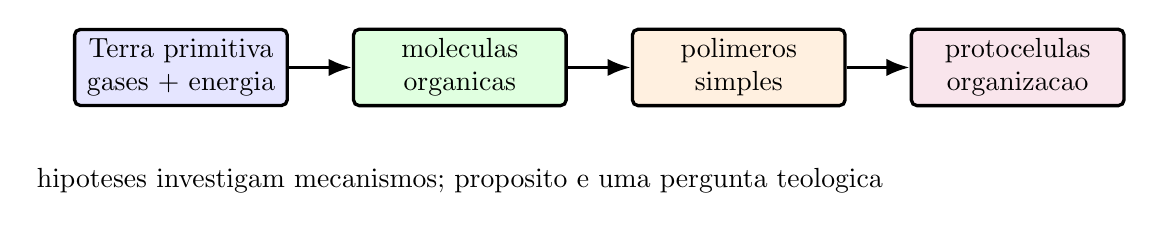
\begin{tikzpicture}[>=Latex,node distance=0.75cm]
  \tikzstyle{box}=[draw,rounded corners=2pt,very thick,align=center,minimum width=2.7cm,minimum height=0.75cm]
  \node[box,fill=blue!10] (terra) {Terra primitiva\\gases + energia};
  \node[box,fill=green!12,right=0.8cm of terra] (mol) {moleculas\\organicas};
  \node[box,fill=orange!12,right=0.8cm of mol] (pol) {polimeros\\simples};
  \node[box,fill=purple!10,right=0.8cm of pol] (proto) {protocelulas\\organizacao};
  \draw[very thick,->] (terra) -- (mol);
  \draw[very thick,->] (mol) -- (pol);
  \draw[very thick,->] (pol) -- (proto);
  \node[align=center,below=0.65cm of mol] {hipoteses investigam mecanismos; proposito e uma pergunta teologica};
\end{tikzpicture}
\end{document}
